\documentclass[tikz,border=4pt]{standalone}
\usepackage[T1]{fontenc}
\usepackage{helvet}
\renewcommand{\familydefault}{\sfdefault}
\usetikzlibrary{positioning,arrows.meta,fit}
\begin{document}
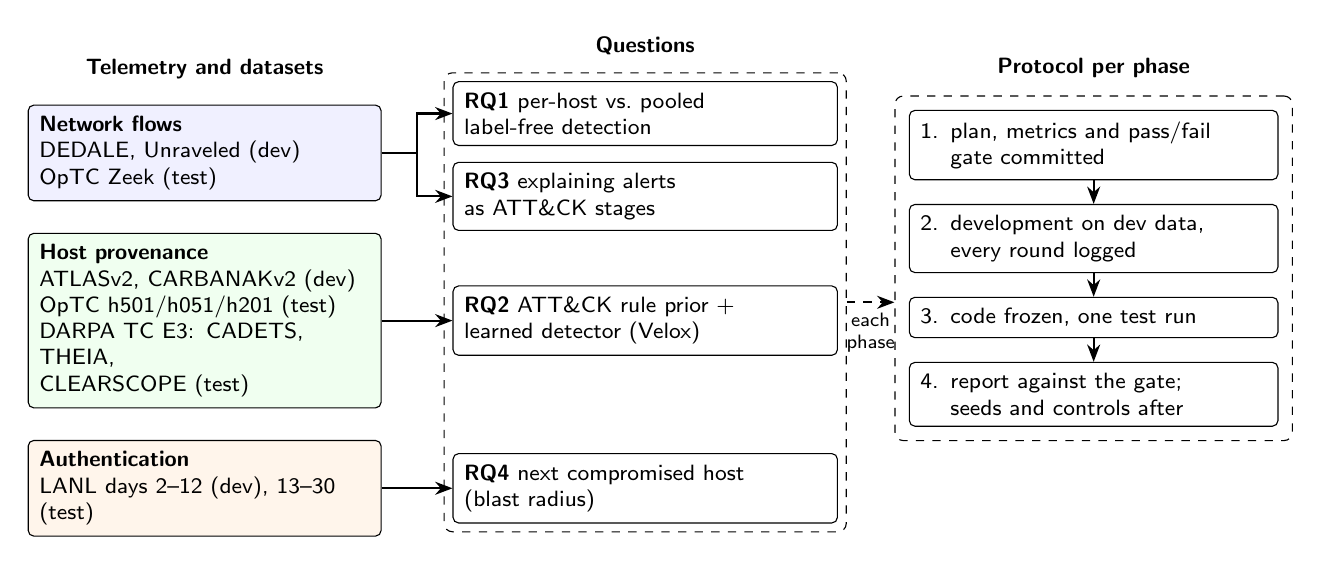
\begin{tikzpicture}[
  font=\footnotesize, node distance=4mm and 9mm,
  box/.style={draw, rounded corners=2pt, align=left, inner sep=4pt, text width=#1},
  box/.default=4.2cm,
  head/.style={font=\footnotesize\bfseries, align=center},
  arr/.style={-{Stealth[length=2.2mm]}, thick}]
% telemetry
\node[head] (h1) {Telemetry and datasets};
\node[box, below=2mm of h1, fill=blue!6] (net) {\textbf{Network flows}\\DEDALE, Unraveled (dev)\\OpTC Zeek (test)};
\node[box, below=of net, fill=green!6] (prov) {\textbf{Host provenance}\\ATLASv2, CARBANAKv2 (dev)\\OpTC h501/h051/h201 (test)\\DARPA TC E3: CADETS, THEIA,\\CLEARSCOPE (test)};
\node[box, below=of prov, fill=orange!8] (auth) {\textbf{Authentication}\\LANL days 2--12 (dev), 13--30 (test)};
% questions
\node[box=4.6cm, right=of net, yshift=5mm] (rq1) {\textbf{RQ1} per-host vs.\ pooled\\label-free detection};
\node[box=4.6cm, below=2mm of rq1] (rq3) {\textbf{RQ3} explaining alerts\\as ATT\&CK stages};
\node[box=4.6cm, right=of prov] (rq2) {\textbf{RQ2} ATT\&CK rule prior +\\learned detector (Velox)};
\node[box=4.6cm, right=of auth] (rq4) {\textbf{RQ4} next compromised host\\(blast radius)};
\draw[arr] (net.east) -- ++(4.5mm,0) |- (rq1.west); \draw[arr] (net.east) -- ++(4.5mm,0) |- (rq3.west);
\draw[arr] (prov) -- (rq2); \draw[arr] (auth) -- (rq4);
% protocol
\node[box=4.4cm, right=of rq1, yshift=-4mm] (p1) {1. plan, metrics and pass/fail\\\phantom{1. }gate committed};
\node[box=4.4cm, below=3mm of p1] (p2) {2. development on dev data,\\\phantom{2. }every round logged};
\node[box=4.4cm, below=3mm of p2] (p3) {3. code frozen, one test run};
\node[box=4.4cm, below=3mm of p3] (p4) {4. report against the gate;\\\phantom{4. }seeds and controls after};
\draw[arr] (p1) -- (p2); \draw[arr] (p2) -- (p3); \draw[arr] (p3) -- (p4);
\node[draw, dashed, rounded corners=3pt, inner sep=5pt, fit=(p1)(p4)] (pbox) {};
\node[draw, dashed, rounded corners=3pt, inner sep=3pt, fit=(rq1)(rq4)] (qbox) {};
\draw[arr, dashed] (qbox.east) -- (pbox.west |- qbox.east) node[midway, below, font=\scriptsize, align=center] {each\\phase};
\node[head, above=1mm of qbox] {Questions};
\node[head, above=1mm of pbox] {Protocol per phase};
\end{tikzpicture}
\end{document}
